%%%%%%%%%%%%%%%%%%%%%%%%%%%%%%%%%%%%%%%%%%%%%%%%%%%%%%%%%%%%%%%%%%%%%%
%%                           SECTION IV
%%%%%%%%%%%%%%%%%%%%%%%%%%%%%%%%%%%%%%%%%%%%%%%%%%%%%%%%%%%%%%%%%%%%%


\chapter{\uppercase {High throughput drug screening of mouse embryonic stem cell-derived neurons}}

\subsubsection*{Abstract}

High-throughput screening (HTS) to identify new drugs for neurological disorders often rely on the use of mouse primary neuronal cultures; however, establishing primary cultures from mice is labor intensive and expensive.  Moreover, most HTS facilities do not allow the use of primary cell lines because of the risks associated with contaminating other cell lines in the facility. In contrast, embryonic stem (ES) cells are permitted in most HTS facilities and can be reliable differentiated into neurons, generating an almost unlimited source of cells for large-scale studies. Thus, ES cell-derived neurons are an excellent model system for performing HTS to identify new therapies for neurological disorders. Here, we developed a high-throughput neuronal culture model via ES cells. Mouse C57BL/J6 ES cells were successfully differentiated into neurons on poly-d-lysine, and immunocytochemistry performed using high-throughput imaging system. These results are promising for the field of neurological disorders and drug discovery.

\section{Mouse Embryonic Stem Cell Culture (Timing: 5 days)}

Mouse embryonic stem (ES) cells are a powerful tool for the scientific discovery because of their ability of almost endless self-renew and potential to differentiate into multiple cell types, including neuronal cell types \cite{Lunn2011}. This pluripotency is a result of the cell type used to derive ES cells, inner mass of a developing blastocyst. As such, ES cells are often co-cultured with feeder cells. The pluripotency is facilitated by a complex pathway involving Wnt/\( \beta \)-catenin signaling and cross-talk between Wnt and LIF, leukemia inhibitory factor \cite{Hao2006,Ogawa2006}. This replaces the need for inhibition of GSK3, which phosphorylates \( \beta \)-catenin marking it for ubiquitin-dependent degradation \cite{Clevers2006,MacDonald2009}, making LIF an essential factor in culturing self-renewing mouse ES cells \cite{Wray2011,Smith1988,Williams1988}.

\subsection{Plating feeder cells for co-culture}

As mentioned above, ES cells are often co-cultured with feeder cells when being maintained as self-renewing pluripotent cells. There are a number of feeder cell types to chose from; however, the most common fibroblasts used as feeder cells are mouse embryonic fibroblast (MEF) and SIM mouse embryoderived thioguanine and ouabain resistant (STO) \cite{Thomas1985,Gail1981}. In this study, we use a genetically modified versus of the STO cell line, SNL 76/7, first established by Dr. Allen Bradley \cite{McMahon1990}. The SNL 76/7 is a unique STO line as it contains the murine LIF gene; thus, LIF does not need to be added to the culture media. 

\begin{enumerate}
\item Coat six 100-mm tissue culture dishes with 0.1\% gelatin for SNL adhesion. Add $\sim$7 ml of gelatin (StemCell Technologies) to each dish and incubate for 30 min at room temperature.
\item Aspirate the gelatin from the dishes and allow them to dry for $\sim$5 min.
\item Culture feeder cells for the ES cells co-culture by plating one vial of Mitomycin C-inactivated SNL (approx. \(2.25 \times 10^7\) cells, 60x concentration) into 60 ml of STO media (see recipe in \textbf{Table \ref{table:4-1}}) and plate onto fixed 100-mm tissue culture dishes.
  \begin{enumerate}
  \item Quick thaw vial at 37$^{\circ}$C using a water bath for $\sim$3 min
  \item Add to 10 ml of STO media
  \item Centrifuge (\( < \)270g for 5 min)
  \item Decant supernatant and resuspend in 60 ml of STO media
  \item Add 10 ml to each plate
  \item Disperse the cells with back and forth motion
  \end{enumerate}
\item Incubate overnight before using (37$^{\circ}$C, 5\% CO\(_2\)). SNL must be plated at least one day before adding ES cells. SNL feeder plates are generally good after plating up to 7 days. 
\end{enumerate}

\subsection{Plating ES cells}

Expansion of ES cell is important for downstream HTS studies. As such, ES cells expansion need to be optimized for individual cell-lines. For C57BL/6J ES cells, the following number of passages is sufficient.

\begin{enumerate}
\item Condition one SNL plate with 10 ml of ES media (see recipe in \textbf{Table \ref{table:4-1}} for at least 2 h before plating ES cells. This allows for LIF expression from the SNL to be added to the ES media, which is required to maintain ES cell pluripotency and ability to self-renew.
\item Defrost 1 vial of ES cell, C57BL/6J, (approx. \(3.5 \times 10^6\) cells) in 37$^{\circ}$C water bath for 3 min. Add to 10 ml of ES media. Transfer to 10 ml of ES media in 15 ml tube and spin down (\( < \)270g for 5 min).
\item Decant supernatant and resuspend in 1 ml of ES media. Add cell suspension of SNL conditioned plates. Disperse the cells with back and forth motion. Incubate the ES cells overnight at 37$^{\circ}$C, 5\% CO\(_2\).
\item 24 h after plating, ES cells form small colonies, \textbf{Figure \ref{Figure 4-1: }A}. Change media with 10 ml of ES media. 48 h after plating, ES cells should be 70-80\% confluent, be careful not to let the ES cells over grow. Condition remaining five SNL plates with ES media for 2 h. Passage cells.
  \begin{enumerate}
  \item Aspirate media, and rinse twice with room temperature sterile 1xPBS. Add 2 ml of TrypLE Express (Life Technologies) and incubate for 5 min. Add 3 ml of ES media to neutralize the trypsin and break the colonies into single cell suspension. Transfer to sterile 15 ml tube and spin down (\( < \)270g, 5 min).
  \item Aspirate supernatant and gently resuspend in 5 ml of ES media. Add 1 ml of cell suspension to each conditioned SNL plate. Disperse the cells with back and forth motion and incubate overnight. Change media next day.
  \end{enumerate}
\item 48 h after passaging, ES cells should be 70-80\% confluent. These cells are ready for differentiation.
\end{enumerate}

\section{Neural Induction (Timing: 7 days)}

To induce differentiation of ES cells into neurons, one method is to separate ES cells from SNL and cultured them in suspension as demonstrated in \textbf{Figure \ref{Figure 4-1: }B}. This can be done one of two ways. The first is several feeder free passages, and the second is by using gelatin coated flasks to separate the SNL feeder cells from ES cells. For HTS purposes, the gelatin technique is used. This saves time and resources.

\begin{enumerate}
\item Once ES colonies are ready for neural induction (day 6), coat one T175 with 20 ml of 0.1\% gelatin for 30 min at room temperature. Aspirate gelatin and allow it to dry for $\sim$5 min.
\item Aspirate ES media from ES cells, and rinse twice with room temperature sterile 1xPBS. Add 2 ml of TrypLE Express and incubate for 5 min. Add 3 ml of CA media (see recipe in \textbf{Table \ref{table:4-1}}) to neutralize the trypsin and break the colonies into single cell suspension.
\item Transfer cells suspension to T175 (approx. 25 ml, 5 ml/plate), and incubate for 30 min at 37$^{\circ}$C, 5\% CO\(_2\). After incubation, SNL should have attached to the surface of the gelatin coated flask while the majority of the ES cells should remain floating. Collect the floating ES cells into 50 ml tube and spin down (\( < \)270g, 5 min). Aspirate supernatant and gently resuspend in 5 ml of CA media.
\item Count the cells using a hemocytometer, or automated cell counter, and plate \(4 \times 10^6\) ES cells per 100-mm bacteriological Greiner Petri dishes.
\item Next day change CA media and split CAs 1:2 by carefully transferring the CA suspension into 50 ml tube (1 plate/tube)\footnotemark. Let CAs settle for at least 3 min. Remove supernatant and resuspend CAs gently with 20 ml of CA media. Mix suspension gently with a 25 ml pipette and plate cells on new dishes. \footnotetext{(1) Splitting CAs is highly depended on number of CAs in suspension, this may vary depending on type of serum/serum replacement. (2) Do not use narrow pipettes to mix suspension to avoid dissociating the CAs. (3) By using new plates, this will further remove any lingering SNL feeder cells.}
\item After 48 h in suspension, change CA media as in step 5, however add RA (retinoic acid) at final concentration of 0.5 mM to CA media. This is another 1:2 split of the CAs, which may be optional depending on CAs density in suspension.  For next four day change CA media without splitting (2 plates/tube) by resuspending each tube with 20 ml CA media with 0.5 mM RA.
\end{enumerate}

\section{Neuron Elongation \& Maturation (Timing: 2+ days)}

ES cell-derived neurons are traditionally plated on poly-dl-orithine/laminin co-coating \cite{Bibel2007,Kiris2011,Wu2012}. This co-coat is feasible for 24-well format; however, for high-throughput screening (HTS) purposes poly-d-lysine coated 96- and 384-well plates are more readily available and less expensive, so we conducted experiments to determine if poly-d-lysine pre-coated 96-well plates (VWR) could be used for neuron elongation and maturation.

\begin{enumerate}
\item (Days Post Differentiation, DPD 0) To dissociate the CAs into single cell suspension, transfer CAs to 50 ml tubes (2 plates/tube), and  wash CAs twice with PBS before trypsinizing.
  \begin{enumerate}
  \item Let CAs settle for $\sim$3 min, then remove supernatant and resuspend CAs gently with 20 ml of 1x PBS. Let CAs settle again for $\sim$3 min, and remove supernatant. Resuspend CAs gently with 5 ml 1x PBS and let settle for $\sim$3 min.
  \item Label and open 1.5/1.6 ml tubes, and carefully transfer CAs at the bottom of 50 ml tubes into them. Spin down quickly for about 5 s, and carefully remove supernatant with pipet tip. Add 1 ml of 0.5\% Trypsin-EDTA (Life Technologies). Vortex and place on heat block for 4 min at 37$^{\circ}$C rotation and 450 rpm. Vortex the tubes and spin down quickly.
  \item Remove supernatant and resuspend CAs in CA media to neutralize trypsin. Dissociate CAs by pipetting up and down (approx. 10 times), and spin down quickly for 5 s. Carefully remove as much supernatant as possible and resuspend in N2 media (see recipe in \textbf{Table \ref{table:4-1}}), which should be made fresh.
  \item Filter cell suspension through 40 \( \mu \)m cell strainer by applying drop by drop\footnotemark, and count cells using automated cell counter, or hemocytometer. \footnotetext{Avoid applying pressure.}
  \end{enumerate}
\item Plate \(9.8 \times 10^4\) cells/well for 96-well plate using sterile hydrospeed in N2 media\footnotemark. \footnotetext{Plating density should be optimized for ES cell lines.}
\item 24 h after plating cells should have attached to the plates as shown in \textbf{Figure \ref{Figure 4-1: }C}. (\emph{optional}) Change the N2 media to further remove trace amounts of FBS.
\item 48 h after plating N2 media should be changed to Complete media (see recipe in \textbf{Table \ref{table:4-1}}). Add the BDNF, brain derived neurotrophic factor, fresh for long term cultures of more than three days. Change Complete media every two to three days.
\end{enumerate}

%%%%%%%%%%%%%%%%%%%%%%%%%%%%%%%%%%%%%%%%%%%%%%%%%%%%%%
\begin{figure}[h]
\centering
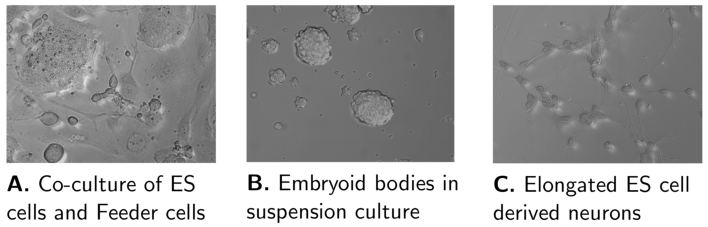
\includegraphics[scale=1.22]{figures/neuron-differentiation2.pdf}
\caption{Differentiation of ES cells into neurons. Light microscope images of \textbf{A)} co-cultures of ES cells and SNL feeder cells at 40x magnification, \textbf{B)} embryoid boides in suspension at 20x magnification, and \textbf{C)} elongated neurons after three days of culture at 20x magnification.}
\label{Figure 4-1: }
\end{figure}
%%%%%%%%%%%%%%%%%%%%%%%%%%%%%%%%%%%%%%%%%%%%%%%%%%%%%%

\section{Representative Results}

\textbf{Figure \ref{Figure 4-2: }} shows an outline of the protocol. The first 5 days involves ES cell culture on SNL feeder cells, which is highly depended on cell lines growth. Following ES cell culture and expansion, the ES cells are separated from the SNL feeder cells expressing LIF to initiate the differentiation process. For high-throughput purposes, cells were grown in suspension and split to avoid overcrowding and obtain optimal numbers. In this case, one vial of ES cells generated $\sim$15-20 plates worth of \(4 \times 10^6 \) cells, which are split twice generating four times the initial number of cells. After neuronal induction, the cellular aggregates are dissociated and placed into serum free N2 media for 48 h. After which, the cells are changed to the Complete media for long term maintenance, with BDNF added to support neuronal growth for cultures lasting more than five days. \textbf{Figure \ref{Figure 4-3: }} shows ES cell-derived neurons that have been cultured for twelve days.

%%%%%%%%%%%%%%%%%%%%%%%%%%%%%%%%%%%%%%%%%%%%%%%%%%%%%%
\begin{figure}
  \centering
  \resizebox{\linewidth}{!}{% Resize table to fit within
    \begin{tikzpicture}[topline/.style={above=3pt,yshift=30pt,text width=6.5cm,font={\LARGE \bfseries}},
      bottomline/.style={below=3pt,yshift=-30pt,text width=6.5cm,font={\LARGE \bfseries}}]
      %draw horizontal line
      \draw[->,shorten >=1pt,>=stealth',line width=4pt] (-0.07,0) -- (30,0);
      %draw vertical lines
      \foreach \x in {0, 10, 24}{
        \draw[line width=4pt] (\x, 20pt) -- (\x,0pt);
      }
      \foreach \x in {2, 14, 28}{
        \draw[line width=4pt] (\x,-20pt) -- (\x,0pt);
      }
      %draw nodes
      \draw (0,0)  node[topline]    {Day 0: Plate Feeder Cells };
      \draw (2,0)  node[bottomline] {Day 1: ES Cell Co-culture};
      \draw (10,0) node[topline]    {Day 5: Neuronal Induction };
      \draw (14,0) node[bottomline] {Day 7: Retinoic Acid Treatment };
      \draw (24,0) node[topline]    {DPD 0: Dissociation of CA };
      \draw (28,0) node[bottomline] {DPD 2: Complete Media };
    \end{tikzpicture}
  }
  \caption{Timeline for the differentiation of ES cells into neurons.}
  \label{Figure 4-2: }
\end{figure}
%%%%%%%%%%%%%%%%%%%%%%%%%%%%%%%%%%%%%%%%%%%%%%%%%%%%%%

%%%%%%%%%%%%%%%%%%%%%%%%%%%%%%%%%%%%%%%%%%%%%%%%%%%%%%
\begin{figure}[!h]
\centering
\begin{tikzpicture}[every label/.style={font=\bfseries}, pic/.style={inner sep=0pt}]
  \node[pic] (nestin) [label={below:Nestin}]                                {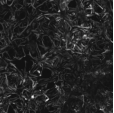
\includegraphics[width=0.25\textwidth]{figures/nestin.pdf}};
  \node[pic] (map2)   [right=0.5mm of nestin,label={below:Map2}]            {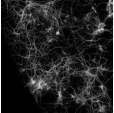
\includegraphics[width=0.25\textwidth]{figures/map2.pdf}};
  \node[pic] (dcx)    [right=0.5mm of map2,label={below:Doublecortin}]      {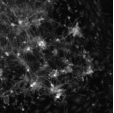
\includegraphics[width=0.25\textwidth]{figures/dcx.pdf}};
  \node[pic] (bTub)   [right=0.5mm of dcx,label={below:$\beta$Tubulin III}] {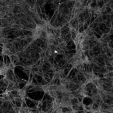
\includegraphics[width=0.25\textwidth]{figures/betaTubulin.pdf}};
\end{tikzpicture}
\caption{High-throughput screening immunofluorescence characterization of differentiated ES cells in 96-well format at day 12, 10x magnification.}
\label{Figure 4-3: }
\end{figure}
%%%%%%%%%%%%%%%%%%%%%%%%%%%%%%%%%%%%%%%%%%%%%%%%%%%%%%

\section{Discussion}

Here, a high-throughput screening method optimized for drug discovery in neuronal cultures is described. For HTS purposes, a large initial number of ES cells is essential; therefore, each individual ES cell-line must be optimized for cell growth. In this method, the use of SNL 76/7 feeder cells is recommended as these cells secrete LIF - supplement required to maintain undifferentiated ES cell state - into the media eliminating the additional purchase of LIF.

For neuronal cultures including ES cell-derived neurons, neural connectivity patterns are crucial for proper function and development. For HTS assays, this adds an additional requirement for an extracellular matrix coating at the bottom of the wells for proper cell attachment and growth \cite{Manthorpe1983,Clark1993,Namba2015}. As such, extra cellular signaling proteins like laminin are needed. The majority of ES cell-derived neuron protocols utilize a co-coat with laminin \cite{Bibel2007,Wu2012}; however, in these protocols the co-coating is applied by hand, which is not conductive to HTS. Furthermore, ordering optical-bottom, sterile plates with a laminin co-coat for 96- or 384-well plates is an expensive special order process that can take upwards to three months.

For those reasons, an alternative solution of using a single coating of poly-d-lysine was choice for this protocol. Poly-d-lysine promotes cell adhesion through ionic interactions \cite{Manthorpe1983}. Moreover, poly-d-lysine is a common substrate choice for culturing primary neurons \cite{Kavalali1999}. In this protocol, we successfully differentiate ES cells into neurons on poly-d-lysine, to the best of our knowledge, for the first time.

Finally, this protocol provides an efficient approach for large-scale differentiation of ES cells into neurons. More importantly, the methods offers a platform for drug discovery for single gene neurological disorders that have mouse models currently available like Angelman syndrome - a severe neurodevelopmental disorder. The power of using ES cells to derive neuron cultures extend beyond the world of drug discovery, especially with the advances in gene manipulation technology (i.e. CRISPR/Cas9 systems), where ES cells can be manipulated in culture before being expanded and differentiated into neurons to answer basic questions in the field of neuroscience. Altogether, this method has the potential to bridge the gap between basic and translational research. 

\section{Materials}

\textit{Equipment}\footnote{All reagents and materials used must be sterile.}

{\setstretch{1.0}
  \begin{enumerate}
  \item Centrifuge
  \item Water bath
  \item Incubator
  \item Microscope
  \item Vortex
  \item Mini Centrifuge
  \item 100-mm Petri dishes
  \item 15 ml \& 50 ml conical tubes
  \item 1.6 ml tubes
  \item Bacteriological Petri dishes
  \item 40 \( \mu \)m nylon cell strainer
  \item Sterile filter 0.2 \( \mu \)m
  \item Poly-d-lysine 96-well pre-coated plates
  \end{enumerate}
}

\pagebreak

%%%%%%%%%%%%%%%%%%%%%%%%%%%%%%%%%%%%%%%%%%%%%%%%%%%%%%
\begin{longtabu} to \textwidth {X[1,l]X[1.4,l]X[1.5,l]X[1.4,r]X[0.8,r]}
  \caption{Media composition}\\
  \label{table:4-1}\\
  \toprule
    \textbf{Media} & \textbf{Components} & \textbf{Company} & \textbf{Cat. \#} & \textbf{Notes}\\
    \midrule
    \endhead
    & SNL 76/7 (untreated) & Applied StemCell, Inc. & ASF-1305 & N.A.\\
    \midrule
    STO Media & KnockOut DMEM & Life Technologies & 10829018 & N.A.\\
    & FBS & & 1600044 & 10\%\\
    & GlutaMAX & & 35050061 & 2 mM\\
    & Penicillin / streptomycin & & 15140122 & 1\%\\
    \midrule
    ES Media & KnockOut DMEM & Life Technologies & 10829018 & N.A.\\
    & FBS & & 1600044 & 10\%\\
    & GlutaMAX & & 35050061 & 2 mM\\
    & Non-essential amino acids & & 111400050 & 1\%\\
    & Penicillin / streptomycin & & 15140122 & 1\%\\
    & \( \beta \)-mercapto- ethanol & Sigma-Aldrich & M6250-100ML & 0.1 mM\\
    \midrule
    CA Media & DMEM & Life Technologies & 11995073 & N.A.\\
    & KnockOut Serum Replacement & & 10828028 & 15\%\\
    & GlutaMAX & & 35050061 & 2 mM\\
    & Non-essential amino acids & & 111400050 & 1\%\\
    & Penicillin / streptomycin & & 15140122 & 1\%\\
    & \( \beta \)-mercapto- ethanol & Sigma-Aldrich & M6250-100ML & 0.1 mM\\
    & Retinoic Acid & & R2625- 50MG & 0.5 mM\\
    \midrule
    N2 Media & DMEM/F-12 & Life Technologies & 11330057 & 1:1\\
    & Neurobasal Medium & & 21103049 & 1:1\\
    & GlutaMAX & & 35050061 & 2 mM\\    
    & B27 & & 17504044 & 1\%\\
    & BSA & Sigma-Aldrich & A7906- 100G & 50 \( \mu \)g/ml\\
    & Progesterone & & P8783-1G & 20 nM\\
    & Putrescence & & P5780-5G & 100 nM\\
    & ITS Supplement & Roche Life Science & 11074547001 & 1\%\\
    \midrule
    Complete Media & Advanced DMEM/F-12 & Life Technologies & 12634028 & 1:1\\
    & Neurobasal Medium & & 21103049 & 1:1\\
    & GlutaMAX & & 35050061 & 2 mM\\
    & B27 & & 17504044 & 1\%\\
    & BDNF & & PHC7074 & 50 ng/ml\\
    \midrule
    MISC & 0.1\% Gelatin & Stem Cell Technologies & 07903 & N.A.\\
    & TrypLE Express & Life Technologies & 12604-021 & N.A.\\
    & 0.5\% Trypsin / EDTA & & 15400054 & N.A.\\
    & PBS & & 10010049 & N.A.\\
    & 100-mm plates & Greiner Bio-One & 633161 & N.A.\\
    & Poly-d-lysine 96-well plates & Thermo Scientific & 152037 & N.A.\\
    \bottomrule
  \end{longtabu}
%%%%%%%%%%%%%%%%%%%%%%%%%%%%%%%%%%%%%%%%%%%%%%%%%%%%%%

\pagebreak

%%%%%%%%%%%%%%%%%%%%%%%%%%%%%%%%%%%%%%%%%%%%%%%%%%%%%%
\begin{longtabu} to \textwidth {X[1.3,l]X[1,l]X[1,r]X[0.7,r]}
  \caption{List of Antibodies}\\
  \toprule
  \textbf{Antibody} & \textbf{Company} & \textbf{Cat. \#} & \textbf{Dilution}\\
  \midrule
  \endhead
  anti-Nestin & EMD Millipore & AB5922   & 1:200\\
  anti-Map2   & Santa Cruz    & sc-20172 & 1:250\\
  anti-DCx    & Biotechnology & sc-8066  & 1:200\\
  anti-mouse (555, Cy3) & Jackson Immuno & 115-165-146 & 1:200\\
  anti-rabbit (488, Cy2) &               & 111-545-144 & 1:200\\
  anti-TOPRO-3 & Life Technologies & T3605 & 1:1000\\
  anti-\( \beta \)Tubulin III & Sigma-Aldrich & T5076 & 1:200\\
  anti-Goat Serum &           & G9023-10ML & 5\%\\
  \bottomrule
\end{longtabu}
%%%%%%%%%%%%%%%%%%%%%%%%%%%%%%%%%%%%%%%%%%%%%%%%%%%%%%
